% Alright so now we're getting into the research paper. No idea what I'm
% doing, but I'm gonna go ahead and riff on it.

% So, requirements of the paper:

% Abstract: I've already written this, but it's pretty garbage. Probably
% going to end up rewriting it.

% Introduction: Present background on the problem (easy). Describe the
% foundation or fundamental concepts (also pretty easy).

% Literature Search: I think I actually need to summarize the key
% results of the papers I've read here. Probably best to start with a
% little theory from Roy, then on to the K-S regularization technique,
% and finishing this with the summary of Davide's switching framework.

% Aspects of Mission of Problem of Interest: Time to setup the
% particular scenario in which I'll be doing the investigation. Probably
% best to just recreate Davide's results, so hyperbolic trajectories wrt
% the third body (Earth), laid out in the heliocentric system. Need to
% discuss

% Importance of the mission (I think these are redundant, and should
% only do one)
% Importance of the problem to astrodynamics
% Development of the solution method
% Analysis of the method

% This will be the meat of the report. Development of the solution
% method should pretty closely follow Davide's paper. Same with
% importance of the particular mission and of the problem. Analysis can
% simply compare the numerical results of the various switching
% techniques.

% Extension: Need to propose extensions to the work. What's a good
% extension here? Another possible mission/scenario? Probably not the
% same asteroid that Davide looked at.

% Looking at the problem of regularized dynamics, it seems that in three 
% dimensional space we're going to need four coordinates, related to the
% original three by the Levi-Civita matrix:

% x = L(u)*u

% Where L is a four by four orthogonal matrix of the parameters u. Going
% from u to x is well defined by this, but going from x to u is not,
% because of the extra coordinate (it's not unique). However, noting
% that the parameter velocity is bilinear to the parameter coordintes,
% we can find a unique transformation that satisfies the original
% relationship.

% The equations of motion are then

% u'' + (K^2/2 - (u',u'))/(u,u)u = Q

% Where Q is the parameterized force. Given a potential for the original
% system, V, we can show that the same potential in parameter space is:

% trans(L(u))*delV/delx = 1/d*delV/delu

% Q = abs(u)^2/2*(-1/2*delV/delu + trans(L(u))*P)

% I still have lingering questions regarding the actual construction of
% V and P. Stiefel appears to treat them as the disturbing potential and
% disturbing force, respectively. But if that's the case, where does the
% original gravitational potential for the main body appear?

\documentclass[11pt,twoside,letterpaper]{article}

\usepackage{amsmath}
\usepackage{graphicx}
\begin{document}
\title{Numerical Integration of Close Encounters in the Circular
  Restricted Three Body Problem}
\author{Jacob Bailey}
\date{December 5, 2018}
\maketitle

\begin{abstract}
  Numerical integration of complex dynamical systems is a nontrivial
  exercise, and presents numerous difficulties to the aspiring
  analyst. The analyst must wrestle not only with the difficulties of
  the physical phenomena arising in the system, but also the numerical
  difficulties of balancing truncation/roundoff error in the
  integrator and quantization effects due to floating point
  represenations in the dynamics functions.

  The problem of three bodies under mutual gravitational attraction is
  one such system. In this paper, we juxtapose the traditional Cowell
  formulation (directly integrating Newton's equations), and a
  regularized formulation due to Kustaanheimo and Steifel;
  investigating their numerical performance and efficiency in treating
  the circular restricted Earth-Sun-Spacecraft problem. 

  \end{abstract}

  \section {Introduction}
  \paragraph{}
    Analytical solutions of the equations of motion for celestial
    bodies have been sought for a number of specific problems and
    general cases for centuries. The combined work of the giants in
    this field are an astrodynamicist’s jewels, for the solutions we
    have to various cases of the two, three, and many body problems
    give significant insight into the behavior of orbits in real
    situations. We draw from these insights whenever we tackle a new
    problem, as guiding principles to lead us on to new solutions.

    However, analytical solutions are incredibly difficult to come by,
    in all but the simplest of problems. Thus, we most often have to
    turn to our computers to look for answers to the more interesting
    questions in astrodynamics. In this paper, we examine the work of
    Davide Amato, Guilio Bau, and Claudio Bombardelli in “Accurate
    orbit propagation in the presence of planetary close encounters”
    \cite{amato_2017}. The topic of planetary close encounters in
    numerically determining a satellite’s trajectory is an interesting
    problem, one fraught with difficulties as the physics the
    spacecraft encounters change significantly throughout different
    portions of its orbit. In using the techniques of regularization
    in the manner of Kustaanheimo and Steifel \cite{stiefel_1971}, we
    show that the overall computational burden of the task can be
    reduced, without sacrificing accuracy in the solutions.
    
  \section{Dynamics, Singularities and Regularization}
  
  \subsection {The Cowell Formulation} 
  To set about the task of numerically integrating our system for the
  restricted three body problem, we first require the equations of
  motion of said system. The most common method of writing these
  equations is via Cowell's formulation; this involves simply summing
  the respective mutual attractions between the N bodies in the
  system, as shown below in \ref{cowell}. 
  
  \begin{equation} \label{cowell}
    \ddot{\vec{r}}_i = \sum_{j=1}^{N} \frac{Gm_j\left(\vec{r}_j - \vec{r}_i\right)}{r_{ij}^3} , i \neq j
  \end{equation}

  Here, \(\ddot{\vec{r}}_i\) is the acceleration of the \textit{i}th
  body in an inertial frame, \(m_j\) is the mass of the \textit{j}th
  body, and \(r_{ij}\) is the magnitude of the relative distance
  between the \textit{i}th and \textit{j}th bodies. The development of
  this formulation is discussed in detail in Roy \cite{roy_2017}.

  It is immediately apparent, upon inspection, that these equations
  contain a few singularities. There are precisely two in this system:
  one when bodies 1 and 2 collide, and another when bodies 2 and 3 do
  the same. This creates difficulties in the numerical solution of the
  system under certain conditions, such as close encounters. An
  adaptive time-step solver, such as the Runge-Kutta-Fehlberg methods,
  would be forced into exceedingly small steps during such a close
  encounter in order to achieve the specified accuracy tolerance,
  leading to undesirably large numbers of steps and function
  evaluations to solve the system. This strategy is thus seen, at
  least at face value, to be less than desirable for some
  applications.
  
  \subsection {Regularization of the Equations of Motion}
  Next, we discuss a method to remove such singularities from the
  equations of motion, without loss of generality/applicability to the
  system. There are other methods of doing so, but here we focus on
  the method originally due to Kustaanheimo, and expounded in the
  monograph by Stiefel and Scheifele \cite{stiefel_1971}. The full
  derivation can be found in said monograph. Here, we discuss briefly
  the salient points of the formulation before presenting it without
  derivation.

  The Kustaanheimo-Stiefel regularized equations of motion are
  achieved via a two step transformation process. The first is a first
  order Sundman transformation to create a fictitious time as the
  independent variable:

  \begin{equation}
    dt = rds
  \end{equation}

  We use this relation to rewrite the equations of motion for the four
  dependent variables \(t, x, y, z\) as functions of the new
  independent variable, \(s\), which corresponds to the eccentric
  anomaly. We note here that \(r\) is the magnitude of the position
  vector.
 
  The second step in the regularization process is what is aptly
  called the K-S tranform. By forming the Levi-Civita matrix with the
  four dimensional parameter vector \(\vec{u}\):
  \begin{equation} \label{levi}
    L(\vec{u}) =
    \begin{bmatrix}
      u_1 & -u_2& -u_3& u_4 \\
      u_2 & u_1 & -u_4& -u_3 \\
      u_3 & u_4 & u_1 & u_2 \\
      u_4 & -u_3& u_2 & -u_1
    \end{bmatrix}
  \end{equation}

  we can transform between the four dimensional parameter space
  \(\vec{u}\) and the three dimensional position space \(\vec{r}\)
  via:

  \begin{equation} \label{xtrans}
    \vec{r} = L(\vec{u})\vec{u}
  \end{equation}

  Taking this transformation to the equations of motion, and using the
  relation of the system energy to the parameter vector, we can then
  write the equations of motion of the system as follows.

  \begin{equation} \label{eom}
    \vec{u}'' + \frac{h_k}{2}\vec{u} = \frac{\mid\vec{u}\mid^2}{2}
    \left(-\frac{1}{2}\frac{\partial{V}}{\partial{\vec{u}}} + L^T\vec{P}\right)
  \end{equation}

  \begin{equation} \label{energy_eom}
    h_k' = \left(\frac{\partial{V}}{\partial{\vec{u}}}, \vec{u}'\right)
    - 2\left(\vec{u}',L^T\vec{P}\right)
  \end{equation}

  \begin{equation} \label{time_eom}
    t' = \left(\vec{u}, \vec{u}\right)
  \end{equation}

  Noting here that \(h_k\) is the Keplerian orbital energy, \(V\) the
  disturbing potential, \(\vec{P}\) the non-potential disturbing
  force, and that prime notation refers to differentiation with
  respect to the fictitious time, \(s\), instead of actual time,
  \(t\). It is worth noting that in this formulation, when the
  disturbing potential and forces are zero (as in the case of
  Keplerian motion), this system reduces to a simple harmonic
  oscillator.

  These regularized equations of motion have increased in total order
  (from order 6 to order 10). However, as we will show, the increase
  in order is a small price to pay for the increase in numerical
  efficiency achieved by removing the singularity at the origin.

  \subsubsection{Transforming Initial Conditions}
  As a consequence of the extra dimension of \(\vec{u}\), there are
  infinitely many \(\vec{u}\) corresponding to any unique
  \(\vec{r}\). As such, we are free to choose any \(\vec{u}\) such
  that equation \ref{xtrans} holds, and the magnitude satisfies the
  relation:

  \begin{equation} \label{umag}
    \mid\vec{r}\mid = \mid\vec{u}\mid^2
  \end{equation}

  Once we have a suitable \(\vec{u}\), we then transform the initial
  velocity of the bodies:

  \begin{equation} \label{initial_velocity}
    \vec{u'}(0) = \frac{1}{2\mid\vec{u}(0)\mid^2}L^T\left(\vec{u}(0)\right)\vec{r'}(0)
  \end{equation}
  
  
  \subsection{Switching Primary Bodies}
  One important point in dealing with the regularized equations of
  motion \ref{eom}-\ref{time_eom} is that not \textit{all} of the
  singularities present in a three body system have been removed. We
  have indeed removed the singularity at the center of the primary
  body, but our disturbing potential will still have a singularity
  when the second and third bodies are very close together.

  A technique to avoid the same numerical difficulties mentioned with
  the Cowell formulation in this case is to employ a change of
  coordinates in the integrating system. At a certain distance
  threshold between the second and third bodies, we can change the
  equations of motion to consider the second body as the primary, and
  the first body as the disturber. Provided the first and second
  bodies are sufficiently distant, as will be the case for the
  specific Sun-Earth-Spacecraft scenario we will investigate here, the
  new equations of motion will no longer be near the singularity in
  the disturbing potential. The larger consequence of this technique
  is that the singularity produced by the proximity of the second and
  third bodies is no longer of importance, since the regularized
  equations of motion are not singular at the origin.

  This technique does require a bit more work, however. Firstly, it is
  common to specify the ``certain distance threshold'' in the real
  coordinates \(\vec{r}\) and/or the real time \(t\). However, we are
  integrating in the parameter space, \(\vec{u}\), and fictitious
  time, \(s\). Thus, some sort of event detection function will be
  necessary to determine at what point during the integration the
  equations of motion should be switched. The techniques developed in
  \cite{amato_2017} will also be employed here for this purpose.

  \section{Numerical Analysis}
  In order to investigate the effectiveness of either dynamical
  formulation in a close encounter situation, we consider a case of
  the circular, restricted three body problem. Specifically, we'll
  investigate the Sun-Earth-Spacecraft system, where the
  infinitesimally small spacecraft will perform a parabolic fly-by of
  Earth, as might happen in a mission involving a gravity assist to
  reach the outer planets of the solar system.

  In both solutions, the Earth and Sun are considered so massive in
  comparison to the spacecraft that we neglect its effect on
  them. Additionally, we also assume that the Earth's orbital
  eccentricity to be sufficiently low for the orbit to be described by
  a circle, with angular velocity equal to the mean motion. This
  reduces the number of equations in the Cowell formulation to 6, with
  the K-S formulation retaining 10.

  Also in both solutions, the initial conditions are the same. We take
  Earth starting at a distance equal to its circular radius along the
  x axis of the coordinates, with the spacecraft's specific position
  and velocity relative to the Earth. These can be stated as follows:

  \begin{equation} \label{ics}
    \vec{r}_{Earth} = r_{Circular}\hat{i}
  \end{equation}
  \begin{equation}
    \vec{\omega}_{Earth} = \omega_{Circular}\hat{k}
  \end{equation}
  \begin{equation}
    \vec{r}_{SC} = 6700\hat{i}
  \end{equation}
  \begin{equation}
    \vec{v}_{SC} = -1\hat{i} + 7\hat{j}
  \end{equation}

  where \(r_{Circular}\) is equal to roughly 149.6 million kilometers,
  and \(\omega_{Circular}\) is roughly 0.0172 radians/day. The
  spacecraft position and velocity are specified in kilometers and
  kilometers/second, respectively. These initial conditions were
  propagated for a total of 546 days, which was roughly the orbital
  period of the spacecraft about the sun. 

  The results of the numerical integration using both schemes are
  shown in figures 1-4. One difference is immediately apparent: the
  orbits for the satellite predicted by each formulation are entirely
  different. The Cowell formulation, shown in figure \ref{cowPath},
  takes more than a year to exit the Earth's Sphere of Influence,
  whereas the KS formulation shows the spacecraft exiting the sphere
  almost immediately, as seen in figure \ref{kspath}.

  \begin{figure}
    \caption{Planar Motion of S/C and Earth in the Cowell formulation}
    \centering
    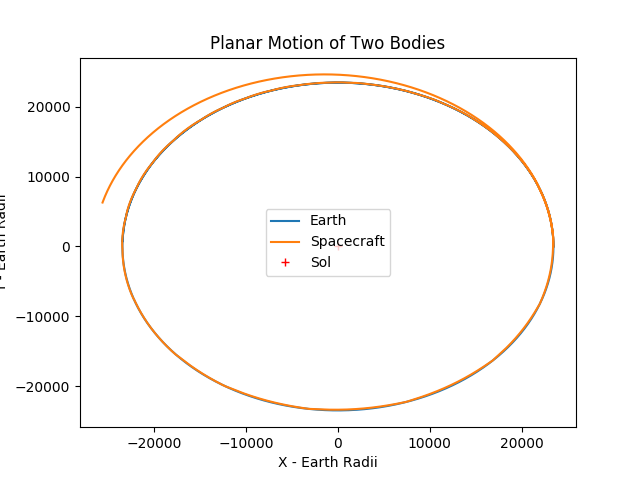
\includegraphics[width=\textwidth]{PlanarPath90}
    \label{cowPath}
  \end{figure}

  \begin{figure}
    \caption{Relative Hamiltonian Error, Cowell}
    \centering
    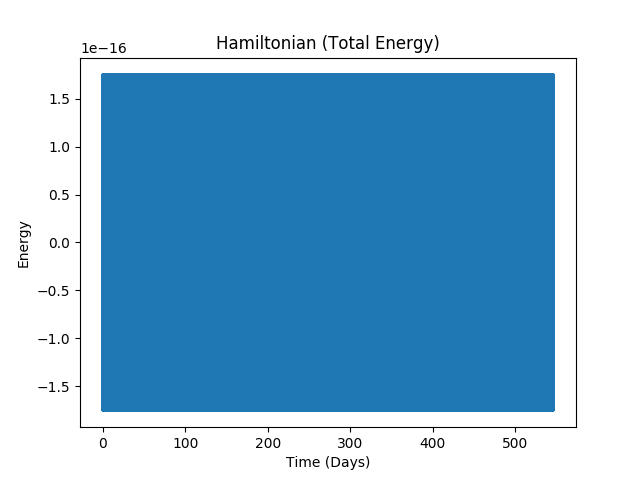
\includegraphics[width=\textwidth]{Hamiltonian90}
    \label{cowHam}
  \end{figure}
  
  The Cowell formulation was actually quite difficult to get to
  converge to a continuous orbit. The time steps necessary for a
  physically possible orbit were on the order of 30 seconds with the
  Cowell formulation, which took an overall 4 minutes and 10.8 seconds
  to complete. The Hamiltonian relative error is shown in figure
  \ref{cowHam}.

  For the KS formulation, the story was completely different. The
  timestep used could be as large as 1 in s (or roughly 1 times the
  semimajor axis of the Earth). This took a whopping 0.647 seconds to
  complete. We note here, that both of these runs were adjusted to
  achieve a similar order of relative error in the Hamiltonian. The
  Hamiltonian relative error is shown in figure \ref{ksham}.

  \begin{figure}
    \caption{Planar Motion of S/C and Earth in the Kustaanheimo-Steifel formulation}
    \centering
    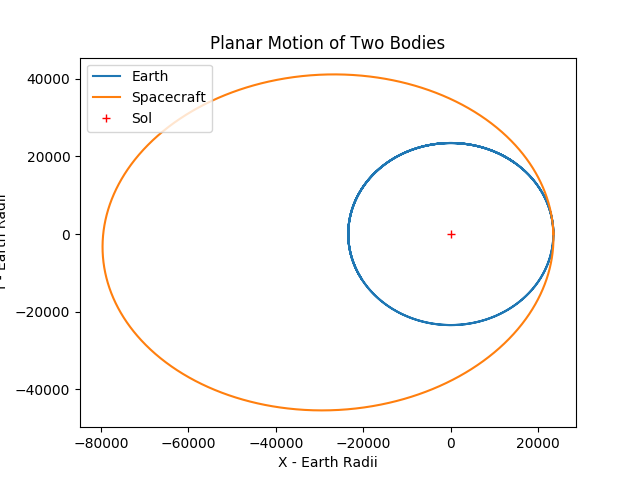
\includegraphics[width=\textwidth]{PlanarPathKS}
    \label{kspath}
  \end{figure}

  \begin{figure}
    \caption{Relative Hamiltonian Error, Kustaanheimo-Steifel}
    \centering
    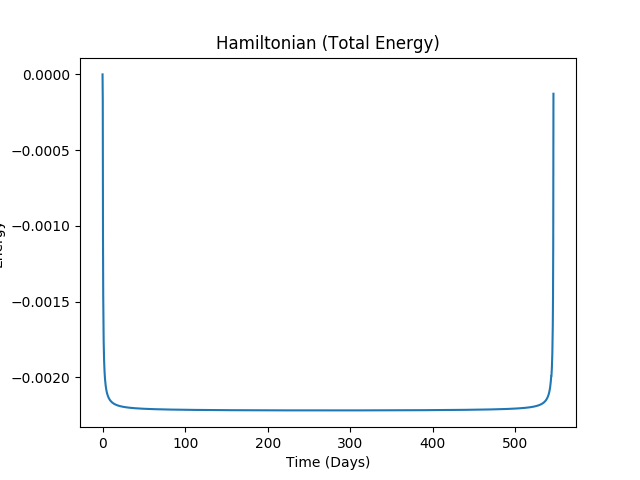
\includegraphics[width=\textwidth]{HamiltonianKS}
    \label{ksham}
  \end{figure}
  
  Also of note is the interesting form of the relative error for the
  KS Hamiltonian. While the Cowell Hamiltonian error was oscillatory,
  the KS Hamiltonian spiked significantly during the close
  encounters. Since the close encounters (rather, where we switch
  primaries at the boundary of the Sphere of Influence) are where we
  expect to see the worst numerical performance due to the singularity
  in the forcing function, this aligns with expectations. To
  succinctly summarize the relative accuracies, we show the magnitude
  of relative errors in the Hamiltonian for both formulations, on
  various time steps, in table \ref{resultsTab}.

  \begin{table}[] \label{resultsTab}
    \centering
    \begin{tabular}{llllll}
      \multicolumn{3}{l}{Cowell} & \multicolumn{3}{l}{Kustaanheimo-Steifel} \\
      dt (s) & RelErr & Run Time & dt (a\_earth) & RelErr & Run Time \\ \hline
      \multicolumn{1}{|l|}{0.1} & \multicolumn{1}{l|}{8e-5} & \multicolumn{1}{l|}{130.4} & \multicolumn{1}{l|}{0.01} & \multicolumn{1}{l|}{2e-3} & \multicolumn{1}{l|}{61.95} \\ \hline
      \multicolumn{1}{|l|}{1} & \multicolumn{1}{l|}{8e-4} & \multicolumn{1}{l|}{13.06} & \multicolumn{1}{l|}{1} & \multicolumn{1}{l|}{2e-3} & \multicolumn{1}{l|}{0.647} \\ \hline
      \multicolumn{1}{|l|}{10} & \multicolumn{1}{l|}{8e-3} & \multicolumn{1}{l|}{0.7} & \multicolumn{1}{l|}{10} & \multicolumn{1}{l|}{8e-3} & \multicolumn{1}{l|}{0.0649} \\ \hline
    \end{tabular}
    \caption{Relative error and run time versus time step, Cowell and KS formulations.}
  \end{table}
  
  \section{Extension of the Work}
  In order to investigate the performance of the KS formulation
  further, we consider changing the switching distance for the
  integrator. In our original formulation, the switching distance was
  set to
  
  \begin{equation}
    \left(\frac{\mu_{Earth}}{\mu_{Sun}}\right)^{\frac{2}{5}}*a_{Earth}\)
  \end{equation}
  
  To look for improvements, we search for a switching distance which
  will minimize the spiking seen in the relative error in the
  Hamiltonian in the original problem. The results are summarized in
  table \ref{switchTable}. We also show the planar path and
  Hamiltonian relative errors in figures \ref{kspath10} and
  \ref{ksham10}, respectively. Of note here is that the time step,
  relative and absolute error tolerances to the solver were all left
  untouched in this variation. 

  \begin{figure}
    \caption{Planar Motion of S/C and Earth}
    \centering
    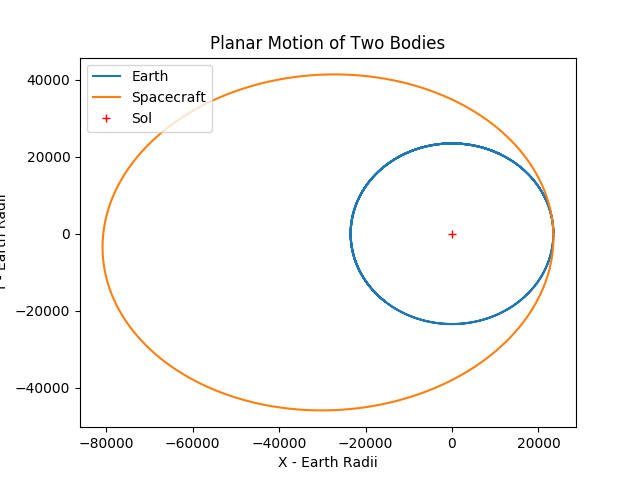
\includegraphics[width=\textwidth]{PlanarPath}
    \label{kspath10}
  \end{figure}

  \begin{figure}
    \caption{Relative Hamiltonian Error, 10x Switching Distance}
    \centering
    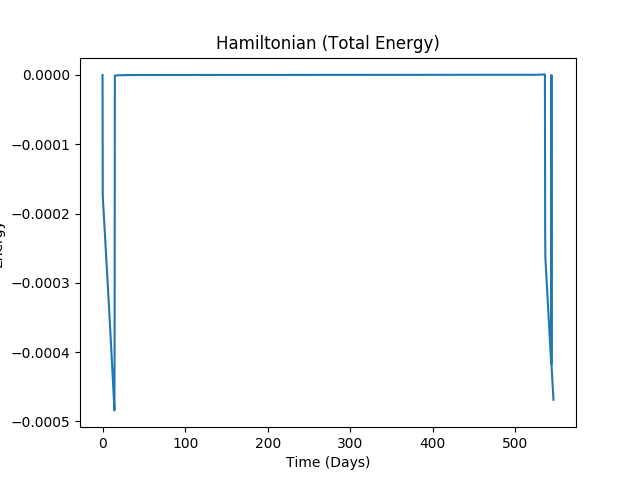
\includegraphics[width=\textwidth]{Hamiltonian}
    \label{ksham10}
  \end{figure}

  \begin{table}[] \label{switchTable}
    \centering
    \begin{tabular}{|l|l|}
      \hline
      Switching Distance & Relative Error \\ \hline
      Original & 2.0e-3 \\ \hline
      10x & 5.0e-4 \\ \hline
      100x & 8.0e-4 \\ \hline
    \end{tabular}
    \caption{Relative Error in the Hamiltonian for different Primary switching distances.}
  \end{table}

  \section{Conclusion}
  Ultimately, we've shown that regularization of the equations of
  motion can be advantageous in numerical propagation of orbits with
  close encounters. While it does suffer from difficulties near
  singularities, far away from them it performs admirably, and with
  far greater efficiency than the Cowell formulation.

  While there are difficulties to consider when using a regularized
  formulation, such as the increased complexity of the equations of
  motion and the spiking of relative errors during close encounters,
  these can be mitigated to some extent. In particular, changing the
  distance from Earth at which we switch the primary bodies, we show
  that the relative error in the Hamiltonian can be reduced further
  for a given time step. Especially when considering long time scale
  problems, or large or highly elliptic orbits, a regularization
  scheme can significantly increase the numerical efficiency of the
  analysis, and reduce the computational burden. 

  \bibliography{bibliography}{}
  \bibliographystyle{plain}
\end{document}

